\documentclass[x11names]{article}
\usepackage{verbatim}
\usepackage{listings}
\usepackage{graphicx}
\usepackage{a4wide}
\usepackage{color}
\usepackage{amsmath}
\usepackage{amssymb}
\usepackage[dvips]{epsfig}
\usepackage[T1]{fontenc}
\usepackage{cite} % [2,3,4] --> [2--4]
\usepackage{shadow}
\usepackage{hyperref}
\usepackage{physics}
\usepackage{url}
\usepackage{tikz}
\usepackage{subcaption}
\usepackage[utf8]{inputenc}
\usepackage{booktabs} % Allows the use of \toprule, \midrule and \bottomrule in tables



%Tikz settings
\usetikzlibrary{shapes,arrows,chains}
% =================================================
% Set up a few colours
\colorlet{lcfree}{Green3}
\colorlet{lcnorm}{Blue3}
\colorlet{lccong}{Red3}
% -------------------------------------------------
% Set up a new layer for the debugging marks, and make sure it is on
% top
\pgfdeclarelayer{marx}
\pgfsetlayers{main,marx}
% A macro for marking coordinates (specific to the coordinate naming
% scheme used here). Swap the following 2 definitions to deactivate
% marks.
\providecommand{\cmark}[2][]{%
  \begin{pgfonlayer}{marx}
    \node [nmark] at (c#2#1) {#2};
  \end{pgfonlayer}{marx}
  } 
\providecommand{\cmark}[2][]{\relax} 



\setcounter{tocdepth}{2}

\lstset{language=c++}
\lstset{alsolanguage=[90]Fortran}
\lstset{basicstyle=\small}
\lstset{backgroundcolor=\color{white}}
\lstset{frame=single}
\lstset{stringstyle=\ttfamily}
\lstset{keywordstyle=\color{red}\bfseries}
\lstset{commentstyle=\itshape\color{blue}}
\lstset{showspaces=false}
\lstset{showstringspaces=false}
\lstset{showtabs=false}
\lstset{breaklines}


\title{ FYS-4411: Computational Physics II \\ Project 3 }
\author{Gullik Vetvik Killie\\
		Håkon Sebastian Bakke Mørk\\
		Jose Emilio Ruiz Navarro
		}

\begin{document}



\maketitle

\abstract{In this work, a simple Variational Monte Carlo (VMC) method has been used to calculate the values of the energies of the ground states of two atoms: Beryllium and Neon. The program uses importance sampling to improve efficiency and make the results more precise. To further improve the efficiency, MPI has been implemented as well. We provide a statistical analysis by the means of blocking so as to not understimate the error of our results. The one-body and charge densities were obtained to compare the effects of the Jastrow factor and provide insight into the electronic structure of the atoms.}

\tableofcontents

\section{Introduction}
VMC methods pose a very attractive alternative to other more complex ways of finding the ground state energies of simple atoms and molecules, like configuration-interaction calculations. The price to be paid in exchange for this simplicity is the sensitivity to the trial wave functions that are used, a VMC algorithm is very sensitive to how these are constructed, so they are one of the most important aspects to be considered (in this work, given the simple nature of the atoms which we will be working with, it's not so important to worry about the quality of the trial wave functions because very simple and basic ones are more than enough to reproduce the actual results). It shouldn't be forgotten that it is a variational method, and this implies that finding the optimal set of variational parameters is going to be the most important part of the calculation itself because it would create a lot of problems if the search range for the parameters was illy defined and not close enough to the variational minimum, namely, the results would have a poor quality in this case. This means that the parameters need to be chosen very carefully, or a recursive search with decreasingly coarse spacing in the space of variational parameters is required if there is no deep knowledge about the system in question.

Instead of evaluating a very complex multidimensional integral to compute the expectation value of an operator, like the hamiltonian in this case, a VMC calculation exploits the fact that the majority of the configuration space where the wave function belongs can be regarded as much less important than other parts, the values of the wave function are too small there and can be mostly ignored during the integration of the algorithm. To capitalize this, the Metropolis algorithm is added to the VMC method, as well as importance sampling.


\section{Theory}


	\subsection{Atoms and Molecules}
	%General atoms stuff that applies to all the different atoms
	The dimensionless hamiltonian for the case of electrons around a nucleus is given by 

	\begin{align}
		\hat{H} &= \sum_{i = 1}^N - \frac{\nabla^2_i}{2} - \frac{Z}{r_i} + \sum_{i < j}\frac{1}{r_{ij}} \label{eq:hamiltonian}
	\end{align}

	where \(r_i\) is the distance from electron \(i\) to the nucleus, \(Z\) is the nucleus charge, and \(r_{ij} = |\vb{r}_i - \vb{r}_j|\).
	The kinetic energy for electron \(i\) is represented by \( - \frac{\nabla^2_i}{2} \), \(- \frac{Z}{r_i}\) the potential energy with respect to the nucleus and \( \frac{1}{r_{ij}} \) the repulsive energy between the electrons \(i\) and \( j\).

	In the VMC calculation the local energy, \(E_L\) is a useful quantity and needs to be finite at all points to be normalizable. So by looking at the limits where the \(E_L\) diverges we can quess the form the wavefunctions should follow.

	\begin{align}
		E_L(r_i,r_{ij}) &= \frac{1}{\Psi_T} \hat{H} \Psi_T
	\end{align}

	In the cases where \(r_i \rightarrow 0\) or \( r_{ij} \rightarrow 0\) we need to make sure that the local energy does not diverge.


		\begin{align}
			\lim_{r_i\rightarrow 0} {E_L(r_i,r_{ij}) } &= \frac{1}{R_i(r_i)} \left( - \frac{1}{2}\pdv[2]{}{x_k} - \frac{Z}{r_i} \right) R_i(r_i) + G(r_i, r_{ij})
			\\
			\lim_{r_i\rightarrow 0} {E_L(r_i,r_{ij}) } &= \frac{1}{R_i(r_i)} \left( - \frac{1}{2}\pdv[2]{}{r_k} - \frac{1}{r_i}\pdv{}{r_i}	 -	 \frac{Z}{r_i} \right) R_i(r_i) + G(r_i, r_{ij})
			\intertext{Given a well behaved wavefunction \( \frac{1}{2}\pdv[2]{}{r_k} \) is finite.}
			\lim_{r_i\rightarrow 0} {E_L(r_i,r_{ij}) } &= 
			\frac{1}{R_i(r_i)} \left( - \frac{1}{r_i}\pdv{}{r_i}	 -	 \frac{Z}{r_i} \right) R_i(r_i)
		\end{align}

		This is finite given when the following differential equation is fulfilled.

		\begin{align}
			\frac{1}{R_i(r_i)} \pdv{}{r_i} R_i(r_i)	=  -Z  \qquad{ \text{ With solution }}  \qquad R_i(r_i) = A e^{-Z}
		\end{align}

		A similar calculation applies for \(r_{12} \rightarrow 0\) and a trialfunction of the form   \[\Psi_T(r_i,r_j,r_{ij}) = e^{ -\alpha \sum_{N}  r_i} \prod^N_{i < j}e^{\beta r_{ij}} = e^{ -\alpha \sum_{N}  r_i} \prod^N_{i < j}e^{\frac{a r_ij}{1 + \beta r_{ij}}} \] should fulfill the condition that the local energy is finite.


	\subsubsection{Helium atom}
		The hamiltonian for the helium atom is given by equation \eqref{eq:hamiltonian}

	\subsubsection{Beryllium atom}

		It is fairly simple to extend the calculational machinery of Variational
		Monte Carlo to other systems than the Helium atom. To show this we
		want to perform calculations on the beryllium atom. As beryllium has
		four electrons compared to the 2 of helium, we need to calculate a
		Slater determinant. However the computation of the Slater determinant
		can be simplified for beryllium. Sticking to hydrogen-like wave functions,
		we can write the trial wave function for beryllium as
		\begin{equation}
			\psi_{T}({\bf r_{1}},{\bf r_{2}},{\bf r_{3}},{\bf r_{4}})=Det\left(\phi_{1}({\bf r_{1}}),\phi_{2}({\bf r_{2}}),\phi_{3}({\bf r_{3}}),\phi_{4}({\bf r_{4}})\right)\prod_{i<j}^{4}\exp{\left(\frac{r_{ij}}{2(1+\beta r_{ij})}\right)},
			\label{eq:BerylliumTrialFunction}
		\end{equation}
		where $Det$ is a Slater determinant and the single-particle wave
		functions are the hydrogen wave functions for the 1s and 2s orbitals.
		With the variational ansatz these are
		\begin{align}
			\phi_{1s}({\bf r_{i}})=e^{-\alpha r_{i}},
		\end{align}
		and
		\begin{align}
			\phi_{2s}({\bf r_{i}})=\left(1-\alpha r_{i}/2\right)e^{-\alpha r_{i}/2}.
		\end{align}
		The Slater determinant is calculated using these ansatzes.

		Furthermore, for the Jastrow factor,
		\begin{align}
			\Psi_{C}=\prod_{i<j}g(r_{ij})=\exp{\sum_{i<j}\frac{ar_{ij}}{1+\beta r_{ij}}},
		\end{align}
		we need to take into account the spins of the electrons. We fix electrons
		1 and 2 to have spin up, and electron 3 and 4 to have spin down. This
		means that when the electrons have equal spins we get a factor
		\begin{align}
			a=\frac{1}{4},
		\end{align}
		and if they have opposite spins we get a factor
		\begin{align}
			a=\frac{1}{2}.
		\end{align}

	\subsubsection{Neon atom}

		Wishing to extend our variational Monte Carlo machinery further we implement Neon. Neon has ten electrons, so it is a big jump from Helium and Beryllium. Therefore we also have to implement a better way to handle the Slater determinant than we did in the previous project. The trial wave function for Neon can be written as
		\begin{equation}
		   \psi_{T}({\bf r_1},{\bf r_2}, \dots,{\bf r_{10}}) =
		   Det\left(\phi_{1}({\bf r_1}),\phi_{2}({\bf r_2}),
		   \dots,\phi_{10}({\bf r_{10}})\right)
		   \prod_{i<j}^{10}\exp{\left(\frac{r_{ij}}{2(1+\beta r_{ij})}\right)},
		   \label{eq:NeonTrialFunction}
		\end{equation}
		Now we need to include the $2p$ wave function as well. It is given as
		\begin{equation}
			\phi_{2p}({\bf r_i}) = \alpha {\bf r_i}e^{-\alpha r_i/2}.
		\end{equation}
		where $ {\bf r_i} = \sqrt{r_{i_x}^2+r_{i_y}^2+r_{i_z}^2}$.

	%Contains a broad overview over the monte carlo method

\subsection{Monte Carlo method with simple Metropolis sampling}
		In a quantum mechanical system the energy is given by the expectation value of the Hamiltonian, let \(\Psi_T\) be a proposal for a wavefunction that can describe the system.

		\begin{align}
			E[\hat{H}] = \expval{\hat{H}}{\Psi_T} = \frac{\int{d\vb{R} \Psi_T^*(\vb{R})\hat{H} \Psi_T(\vb{R})  }}{ \int{d\vb{R} \Psi_T^*(\vb{R}) \Psi_T(\vb{R}) }}
		\end{align}

		Let us introduce a local energy:

		\begin{align}
			E_L(\hat{H}) &= \frac{1}{ \Psi_T(\vb{R}) } \hat{H} \Psi_T(\vb{R}))
		\end{align}

		\begin{align}
			E[\hat{H}] &= \frac{\int{d\vb{R} \Psi_T^*(\vb{R}) \Psi_T(\vb{R}) E_L(\vb{R}))  }}{ \int{d\vb{R} \Psi_T^*(\vb{R}) \Psi_T(\vb{R}) }}
			\intertext{Since the denumerator is a scalar constant after integrating it we can put it inside the integral in the numerator}
			E[\hat{H}] &= \int{d\vb{R} \frac{\Psi_T^*(\vb{R}) \Psi_T(\vb{R})  }{\int{d\vb{R'} \Psi_T^*(\vb{R'}) \Psi_T(\vb{R'})}}  E_L(\vb{R})  }
			\\
			E[\hat{H}] &= \int{d\vb{R} P(\vb{R}) E_L(\vb{R}) }
		\end{align}

		This probability function with \(P(\vb{R})\) as the pdf, and we can use Monte Carlo integration to solve the integral. The algorithm for a Monte Carlo integration is given below.

		\begin{enumerate}
			\item Initialise system. Give particles a random position and decide how many Monte Carlo Cycles to run.
			\item Start Monte Carlo Calculations
				\begin{enumerate}
					\item Propose a move of the particles according to an algorithm, for example \newline \( \vb{R_{new}} = \vb{R_{old}} + \delta * r \), where \(r\) is a random number in \([0,1]\)
					\item Accept or reject move according to \( P(\vb{R_{new}})/ P(\vb{R_{old}}) \ge r \), where r is a new number. Update position values if accepted.
					\item Calculate energy for this cycle.
				\end{enumerate}
		\end{enumerate}

		See the git reposity in the reference list for a implementation of the Monte Carlo algorithm.

	%Contains the blocking and MPI parts of the theory
\subsubsection{Importance sampling}
		We now want to make the code more efficient, so we replace the brute
		force Metropolis algorithm with a walk in coordinate space biased
		by the trial wave function, an approach based on the Fokker-Planck
		equation and the Langevin equation for generating a trajectory in
		coordinate space.

		For one particle or walker, a diffusion process characterized by a
		time-dependent probability density $P\left(x,t\right)$ in one dimension
		we have the Fokker-Planck equation
		\begin{align}
			\frac{\partial P}{\partial t}=D\frac{\partial}{\partial x}\left(\frac{\partial}{\partial x}-F\right)P\left(x,t\right),
		\end{align}
		where $F$ is a drift term and $D$ is the diffusion coefficient.

		The new positions in coordinate space are found using the Langevin
		equation with Euler's method. We go from the Langevin equation
		\begin{align}
			\frac{\partial x(t)}{\partial t}=DF(x(t))+\eta
		\end{align}
		where $\eta$ is a random variable. This gives us a new position
		\begin{align}
			y=x+DF(x)\Delta t+\xi\sqrt{\Delta t}.
		\end{align}
		Here $\xi$ is gaussian random variable and $\Delta t$ is a chosen
		time step. $D$ comes from the factor $1/2$ in the kinetic energy
		operator, and is therefore equal to $1/2$ in atomic units.

		The process of isotropic diffusion characterized by a time-dependent
		probability density $P\left(\mathbf{x},t\right)$ will, as an approximation,
		obey the Fokker-Planck equation
		\begin{align}
			\frac{\partial P}{\partial t}=\sum_{i}D\frac{\partial}{\partial\mathbf{x_{i}}}\left(\frac{\partial}{\partial\mathbf{x_{i}}}-\mathbf{F_{i}}\right)P(\mathbf{x},t),
		\end{align}
		where $\mathbf{F}_{i}$ is component number $i$ of the drift term
		caused by an external potential, and $D$ is the diffusion coefficient.
		We set the left hand side equal to zero and obtain the convergence
		to a stationary probability density
		\begin{align}
			\frac{\partial^{2}P}{\partial{\mathbf{x_{i}}^{2}}}=P\frac{\partial}{\partial{\mathbf{x_{i}}}}\mathbf{F_{i}}+\mathbf{F_{i}}\frac{\partial}{\partial{\mathbf{x_{i}}}}P.
		\end{align}


		Inserting the drift vector, $\mathbf{F}=g(\mathbf{x})\frac{\partial P}{\partial\mathbf{x}}$,
		we get
		\begin{align}
			\frac{\partial^{2}P}{\partial{\mathbf{x_{i}}^{2}}}=P\frac{\partial g}{\partial P}\left(\frac{\partial P}{\partial{\mathbf{x}_{i}}}\right)^{2}+Pg\frac{\partial^{2}P}{\partial{\mathbf{x}_{i}^{2}}}+g\left(\frac{\partial P}{\partial{\mathbf{x}_{i}}}\right)^{2}
		\end{align}
		To meet the condition of stationary density the left hand side has
		to be zero. This means that the terms containing first and second
		order derivatives has to cancel each other, which is only possible
		if $g=\frac{1}{P}$. This yields
		\begin{align}
			\mathbf{F}=2\frac{1}{\Psi_{T}}\nabla\Psi_{T},
		\end{align}
		known as the quantum force. This so-called force pushes the walker
		towards regions of configuration space where the trial wave function
		is large, thus increasing the efficiency of the simulation. This is
		a great improvement on the Metropolis algorithm where the walker has
		the same probability to move in every direction.

		From the Fokker-Planck equation we get a transition probability given
		by Green's function
		\begin{align}
			G(y,x,\Delta t)=\frac{1}{(4\pi D\Delta t)^{3N/2}}\exp\left(-\frac{(y-x-D\Delta tF(x))^{2}}{4D\Delta t}\right)
		\end{align}
		This means that the Metropolis algorithm
		\begin{align}
			A(y,x)=\mathrm{min}(1,q(y,x))),
		\end{align}
		where
		\begin{align}
			q(y,x)=\frac{|\Psi_{T}(y)|^{2}}{|\Psi_{T}(x)|^{2}},
		\end{align}
		is replaced by the Metropolis-Hastings algorithm,
		\begin{align}
			q(y,x)=\frac{G(x,y,\Delta t)|\Psi_{T}(y)|^{2}}{G(y,x,\Delta t)|\Psi_{T}(x)|^{2}}
		\end{align}


\subsection{Implementation of MPI}
		As the calculations now become increasingly complex and heavy we implement MPI to make use of multiple processors. Personal computers today usually have two, four or sometimes eight processors, which will give a fairly good speedup to our calculations. With bigger atoms or systems it is crucial to implement a way to distribute calculation to multiple processors.

		Implementing MPI in the Monte Carlo method is very easy. As we deal with statistical values we can easily split up the problem. Each process will run its own set of samples. The number of samples used by each process is simply $n/p$, where $n$ is the total number of samples we want to do, and $p$ is the number of processes. In the end all processors send their results to the master process, which sums up the values and takes the average over all processes.

	\subsection{Blocking}
	\label{sec:blocking}
		Blocking refers to a method to more accurately estimate the error of the values obtained by the VMC algorithm. It is and independent method from the VMC computation that can be used afterwards to get a more robust estimate of the variance. The basic idea lies on the correlations between all the measurements. If these are important enough, they will produce an increase in the error that needs to be taken into account. The reason behind this is related to the effective amount of measurements, if there are correlations there will be measurements that will contain less information, so these won't be as valuable as the rest and it will be as if there are \textit{less} measurements than we actually have. Obviously this is a problem, the usual identification of the error with $\sqrt{\frac{\sigma}{n}}$ will be overly optimistic and a correction is needed.

		\begin{align}
			f_d=\frac{1}{n-d}\sum_{k=1}^{n-d}{\left(x_k-\bar{x}_n\right)\left(x_{k+d}-\bar{x}_n\right)}
		\end{align}

		Where $f_d$ is the correlation between measurements separated by a distance of $d$. This can be used to give an actual form to the correction factor:\\

		\begin{align}
			\tau=1+2\sum_{d=1}^{n-1}{\frac{f_d}{var\left(x\right)}}
		\end{align}

		This is the autocorrelation time and it relates the error with the variance:\\

		\begin{align}
			err^2=\frac{\tau}{n}var\left(x\right)
		\end{align}

		And the inverse of the first factor is  the number of effective measurements (that are useful since they contain information):\\

		\begin{align}
			n_{eff}=\frac{n}{\tau}
		\end{align}

		The expression that relates the standard deviation with this correlation time is thus:\\

		\begin{align}
			\sigma=\sqrt{\left(\frac{1+2\tau/\Delta t}{n}\left(\bar{x^2}-\bar{x}^2\right)\right)}
		\end{align}

		Where $\Delta t$ is the time between samples, and it's commonly smaller than $\tau$. The main problem is that to compute $\tau$ a lot of time is needed, and this is not feasible in most cases.\\

		The solution is to use blocking, and the algorithm to do this is quite simple. The total amount of measurements is divided into blocks of a certain size, and for each block the standard deviation is obtained. When the standard deviation stops increasing as the block size does, the correlations are irrelevant and the value for it is ready.\\

	\subsection{Energy minimization}
		As it can be expected, the values of the energy can depend heavily with respect to the variational parameters, so the optimal value must be found. This usually means finding the minimum value, and the first option would obviously be just a brute force search, but this is not efficient and there are better alternatives. Among these, we can find the steepest descent method, the conjugate gradient method and the Newton-Raphson method (also known as just Newton's method). The first two offer the possibility of finding a minimum in a multivariate space, while Newton's method only allows searching in one dimension, but is simpler and faster.\\

		Since these methods don't find minima but the zeros of a function, the derivative of said function is needed. But there is no analytical expression for the local energy, so a workaround must be used. It is possible to find an analytical expression of this derivative as a function of the values of the local energy and the logarithmic derivative of the wave function. Following \parencite{mortens_notes} section $16.11$ the expression for the derivative with respect to parameter $c$ is:\\

		\begin{equation}\frac{\partial E}{\partial c}=2\left[\langle E_L\frac{\partial\ln{\Psi}}{\partial c}\rangle-E\langle\frac{\partial\ln{\Psi}}{\partial c}\rangle\right]\end{equation}

		Or more explicitly:\\

		\begin{equation}\frac{\partial E}{\partial c}=\frac{2}{N}\left[\sum_{i=1}^N\left(\left[E_L\left(c\right)\right]_i\left[\frac{\partial\ln{\Psi}}{\partial c}\right]_i\right)-\frac{1}{N}\sum_{i=1}^N\left(\left[E_L\left(c\right)\right]_i\sum_{j=1}^N\left[\frac{\partial\ln{\Psi}}{\partial c}\right]_j\right)\right]\end{equation}

		Where the indices's $i$ and $j$ run through all the timesteps independently of each other. In our case, we are going to derive with respect to $\beta$ only, because we are only interested in minimization in that direction. Since the derivative is composed of three parts, two for the Slater determinants and one for the Padé-Jastrow interaction part, we get:\\

		\begin{equation}\frac{\partial\ln{\Psi}}{\partial\beta}=\frac{\partial\ln{\Psi_{SD\uparrow}}}{\partial\beta}+\frac{\partial\ln{\Psi_{SD\downarrow}}}{\partial\beta}+\frac{\partial\ln{\Psi_J}}{\partial\beta}=\frac{\partial\ln{\Psi_J}}{\partial\beta}=\frac{\partial\left(\sum_{i<j}\frac{ar_{ij}}{1+\beta r_{ij}}\right)}{\partial\beta}=\sum_{i<j}\frac{-ar_{ij}^2}{\left(1+\beta r_{ij}\right)^2}\end{equation}

		So the resulting expression is:\\

		\begin{equation}\frac{\partial E}{\partial\beta}=\frac{2}{N}\left[\sum_{i=1}^N\left(\left[E_L\left(\beta\right)\right]_i\left[\sum_{k<l}\frac{-ar_{kl}^2}{\left(1+\beta r_{kl}\right)^2}\right]_i\right)-\frac{1}{N}\sum_{i=1}^N\left(\left[E_L\left(\beta\right)\right]_i\sum_{j=1}^N\left[\sum_{k<l}\frac{-ar_{kl}^2}{\left(1+\beta r_{kl}\right)^2}\right]_j\right)\right]\end{equation}

		With $k$ and $l$ running through the electrons. Newton's method will be used for its simplicity, and because we will only work with $\beta$. This method additionally requires the derivative of the function ($\frac{\partial E}{\partial\beta}$ in this case), but it's not possible to simply derive with respect to $\beta$ again because there is no analytical expression for $E_L\left(\beta\right)$, so we must resort to numerical derivation. A simple, first oder finite difference method can be used for this:\\

		\begin{equation}\frac{\partial^2 E}{\partial\beta^2}=\lim_{h\to 0}\frac{\frac{\partial^2 E\left(\beta+h\right)}{\partial\beta^2}-\frac{\partial^2 E\left(\beta\right)}{\partial\beta^2}}{h}\end{equation}

		And with this Newton's method can be implemented in a straight forward manner with one simple equation:\\

		\begin{equation}\beta_{i+1}=\beta_i-\frac{\frac{\partial E}{\partial\beta}}{\frac{\partial^2 E}{\partial\beta^2}}\end{equation}

		The index $i$ represents the iterations of Newton's method, not the iterations of the Monte Carlo loop, for each iteration of this index, a whole Monte Carlo loop is performed. In iteration $0$ a seed must be provided. Depending on the guess for this seed, the method's performance will be better or worse.\\

		There is one catch, the values of the first derivative are computed as a part of the Monte Carlo loop, and are thus susceptible to a certain degree of randomness. This variability introduces some uncertainty in each iteration. Basically, we are not applying the method to a function, but to a scattered point cloud from which we sample points one at a time. This, coupled with the fact that the second derivative is obtained numerically from two points of that cloud, made the method show poor results, namely slow convergence to values that apparently depended heavily on the seed choice. To circumvent this issue, a different, yet similar method was used.\\

		The bisection method is similar to Newton-Raphson method, but it only needs the function that has the roots we want to find. And, instead of a point seed, it needs an interval seed. The method exploits Bolzano's theorem in said interval: if the values of the function (the derivative of the local energy in this case) in the extremes have different signs, the existence of at least one root is guaranteed. By evaluating the function in the midpoint of the interval, it's possible to know in which half of it the root lies, and thus the interval can be reduced to one of its halves. This process is repeated until a certain tolerance is reached and the root is obtained. In our case we don't have to worry about multiple roots because we know that there is only one minimum, the only problem is choosing the appropriate intervals so that the method can find the root.\\

		\begin{figure}
			\centering \includegraphics[width=0.45\linewidth]{../figures/Bisection_method}
			\protect\caption{Schematic representation of the bisection method: in each iteration the interval is halved in two and it converges linearly to the solution}
		\end{figure}

		The main advantage here compared to Newton's method is that the sensibility to the values of the function is much smaller because only the sign of the function values is important (and this only becomes a problem when we are already very close to the root). The other advantage is the robustness and simplicity, the method will converge no matter what if the appropriate interval is chosen, which is not something very complicated to guess and can be checked quite fast in case it's not so obvious. The downside is the linear, comparatively slow convergence; but in this case, due to the the imprecision in obtaining the values of the derivative of the local energy, Newton's method becomes relatively slow as well, so it's not actually a problem for our purposes.\\


	

	\subsection{Derivation of local energies}
		The local energy of is dependant on the Hamiltonian and the wavefunction describing the system, the Hamiltonian incorporates both a kinetic energy part given by \( \frac{\nabla_i^2}{2} \) for each particle
		and a potential energy part given by \(\frac{Z}{r_i}\) and \(\frac{1}{r_{ij}}\), where \(Z\) is the charge of the center, \(r_i\) is the distance for electron \(i\) to the atom center and \(r_{ij}\) is the distance between electron \(l\) and \(m\). Then the local energy is given by the following:

		\begin{align}
			E_L &= \sum_{i,i<j}{\frac{1}{ \Psi_T(\vb{r_i} , \vb{r_{ij}}) } \hat{H} \Psi_T(\vb{r_i} , \vb{r_{ij}})}
			\\
			&=	\sum_{i,i<j}\frac{1}{ \Psi_T(\vb{r_i} , \vb{r_{ij}}) } \left( - \frac{\nabla_i^2}{2} -\frac{Z}{r_i}  -  \frac{Z}{r_j} +  \frac{1}{r_{ij} }  \right) \Psi_T(\vb{r_i} , \vb{r_{ij}})
			\\
			&= \sum_{i,i<j}{-\frac{1}{2\Psi_T} \left(\nabla_i^2 \Psi_T  \right)  -\frac{Z}{r_i}  -  \frac{Z}{r_j} +  \frac{1}{r_{ij} }}
		\end{align}

		Let us change derivation variables:

		\begin{align}
			-\frac{1}{2\Psi_T} \left(\nabla_i^2 \Psi_T  \right) &= \sum_{m=1}^{3}{-\frac{1}{2\Psi_T} \left( \pdv[2]{\Psi_T}{x_m} \right)_i}
			\\
			&= \sum_{m=1}^{3}{-\frac{1}{2\Psi_T} \left( \pdv{}{x_m} \left( \pdv{\Psi_T}{r_i}\pdv{r_i}{x_m} \right) \right)_i}
			\intertext{Since \(r_i = \left( x_1^2 + x_2^2 + x_3^2 \right)^{1/2}\) then \( \pdv{r_i}{x_m} = \pdv{\left( x_1^2 + x_2^2 + x_3^2 \right)^{1/2}}{x_m} =\frac{x_m}{r_i} \)}
			&= \sum_{m=1}^{3}{-\frac{1}{2\Psi_T} \left( \pdv{}{x_m} \left( \pdv{\Psi_T}{r_i}\frac{x_m}{r_i} \right) \right)_i}
			\\
			&= \sum_{m=1}^{3}{-\frac{1}{2\Psi_T} \left( \pdv{\Psi_T}{x_m}{r_i}\frac{x_m}{r_i} + \pdv{\Psi_T}{r_i} \pdv{}{x_m} \left(\frac{x_m}{r_i} \right) \right)_i}
			\intertext{ The term \( \pdv{}{x_m} \left(\frac{x_m}{r_i} \right) \) becomes for the different values for \(m\),  \(\pdv{}{x_1}  \left( \frac{x_1}{\left( x_1^2 + x_2^2 + x_3^2 \right)^{1/2}} \right) = \frac{x_2^2 + x_3^2}{r_i^3}\) so all the values for \(m\) term it should sum up to \( \frac{ 2 (x_1^2 + x_2^2 + x_3^2) }{ r_i^3 } \) }
			&= -\frac{1}{2\Psi_T} \left( \pdv[2]{\Psi_T}{r_i}\frac{x_1^2 + x_2^2 + x_3^2}{r^2_i} + \pdv{\Psi_T}{r_i} \frac{ 2 (x_1^2 + x_2^2 + x_3^2) }{ r_i^3 } \right)_i
			\\
			&= -\frac{1}{2\Psi_T} \left( \pdv[2]{\Psi_T}{r_i} + \pdv{\Psi_T}{r_i} \frac{ 2 }{ r_i } \right)
		\end{align}
		Then the local energy becomes:
		\begin{align}
			E_L = \sum_{i,i<j}{  -\frac{1}{2\Psi_T} \left( \pdv[2]{\Psi_T}{r_i} + \pdv{\Psi_T}{r_i} \frac{ 2 }{ r_i } \right)  -\frac{Z}{r_i}  -  \frac{Z}{r_j} +  \frac{1}{r_{ij} }} \label{eq:localEnergy}
		\end{align}

		We can apply this to the simple helium trialfunction with no electronic interaction to obtain the local energy.

		\subsubsection{Helium: Simple trialfunction}
		The simple version of the trial function is only dependant on one parameter \( \alpha \) and does not take into account interaction between the two electrons, it is of the form
		\[ \Psi_T (\vb{r_1}, \vb{r_2}) = \exp{ -\alpha (r_1 + r_2) } \]Let us set this trialfunction into the equation for the local energy \eqref{eq:localEnergy}.
		\begin{align}
			E_L &= \sum_{i,i<j}{  -\frac{1}{2\Psi_T} \left( \pdv[2]{e^{-\alpha (r_i + r_j)}}{r_i} + \pdv{e^{-\alpha (r_i + r_j)}}{r_i} \frac{ 2 }{ r_i } \right)  -\frac{Z}{r_i}  -  \frac{Z}{r_j} +  \frac{1}{r_{ij} }}
			\\
			E_L &= -\frac{1}{2\Psi_T} \sum_{i=1}^2{ \left( \alpha^2 -\alpha \frac{ 2 }{ r_i } \right) \Psi_T  -\frac{Z}{r_i} +  \frac{1}{r_{ij} } }
			\\
			E_L &= -\alpha^2 + (\alpha-Z) \left( \frac{1}{r_1} + \frac{1}{r_2} \right) + \frac{1}{r_{12}} \label{eq:heliumLocalEnergy}
		\end{align}

	\subsection{Calculating the Slater determinant}
		\subsubsection{Setting up the Slater determinant}
			To describe the wavefunction of multiple fermions we use a Slater
			determinant. The Slater determinant has the form
			\begin{align}
				\Phi(\mathbf{r}_{1},\mathbf{r}_{2},\mathbf{r}_{3},\mathbf{r}_{4},\alpha,\beta,\gamma,\delta)=\frac{1}{\sqrt{4!}}\left|\begin{array}{cccc}
				\psi_{100\uparrow}(\mathbf{r}_{1}) & \psi_{100\uparrow}(\mathbf{r}_{2}) & \psi_{100\uparrow}(\mathbf{r}_{3}) & \psi_{100\uparrow}(\mathbf{r}_{4})\\
				\psi_{100\downarrow}(\mathbf{r}_{1}) & \psi_{100\downarrow}(\mathbf{r}_{2}) & \psi_{100\downarrow}(\mathbf{r}_{3}) & \psi_{100\downarrow}(\mathbf{r}_{4})\\
				\psi_{200\uparrow}(\mathbf{r}_{1}) & \psi_{200\uparrow}(\mathbf{r}_{2}) & \psi_{200\uparrow}(\mathbf{r}_{3}) & \psi_{200\uparrow}(\mathbf{r}_{4})\\
				\psi_{200\downarrow}(\mathbf{r}_{1}) & \psi_{200\downarrow}(\mathbf{r}_{2}) & \psi_{200\downarrow}(\mathbf{r}_{3}) & \psi_{200\downarrow}(\mathbf{r}_{4})
				\end{array}\right|
			\end{align}
			for a four-fermionic system. Because the spatial wave functions for
			spin up and spin down states are equal, this Slater determinant equals
			zero. We can rewrite the Slater determinant as a product of two Slater
			determinants, one for spin up and one for spin down. This gives us
			\begin{eqnarray*}
				\Phi(\mathbf{r}_{1},\mathbf{r}_{2},,\mathbf{r}_{3},\mathbf{r}_{4},\alpha,\beta,\gamma,\delta) & = & \det\uparrow(1,2)\det\downarrow(3,4)-\det\uparrow(1,3)\det\downarrow(2,4)\\
		 		&  & -\det\uparrow(1,4)\det\downarrow(3,2)+\det\uparrow(2,3)\det\downarrow(1,4)\\
		 		&  & -\det\uparrow(2,4)\det\downarrow(1,3)+\det\uparrow(3,4)\det\downarrow(1,2)
			\end{eqnarray*}
			Here we have defined the Slater determinant for spin up as
			\begin{align}
				\det\uparrow(1,2)=\frac{1}{\sqrt{2}}\left|\begin{array}{cc}
				\psi_{100\uparrow}(\mathbf{r}_{1}) & \psi_{100\uparrow}(\mathbf{r}_{2})\\
				\psi_{200\uparrow}(\mathbf{r}_{1}) & \psi_{200\uparrow}(\mathbf{r}_{2})
				\end{array}\right|
			\end{align}
			and the Slater determinant for spin down as
			\begin{align}
				\det\downarrow(3,4)=\frac{1}{\sqrt{2}}\left|\begin{array}{cc}
				\psi_{100\downarrow}(\mathbf{r}_{3}) & \psi_{100\downarrow}(\mathbf{r}_{4})\\
				\psi_{200\downarrow}(\mathbf{r}_{3}) & \psi_{200\downarrow}(\mathbf{r}_{4})
				\end{array}\right|
			\end{align}
			And the total determinant is of course still zero.

			Further, it can be shown that for the variational energy we can approximate
			the Slater determinant as
			\begin{align}
				\Phi(\mathbf{r}_{1},\mathbf{r}_{2},\dots\mathbf{r}_{N})\propto\det\uparrow\det\downarrow
			\end{align}
			We now have the Slater determinant as a product of two determinants,
			one containing the electrons with only spin up, and one containing
			the electrons of spin down. This approach has certain limits as the
			ansatz isn't antisymmetric under the exchange of electrons with opposite
			spins, but it gives the same expectation value for the energy as the
			full Slater determinant as long as the Hamiltonian is spin independent.
			We thus avoid summing over spin variables.

		\subsubsection{Calculation of the Slater determinant}
			Now we have the Slater determinant written as a product of a determinant
			for spin up and a determinant for spin down. The next step is to invert
			the matrices using LU decomposition. We can thus rewrite a matrix
			$\hat{A}$ as a product of two matrices, $\hat{B}$ and $\hat{C}$
			\[
			\left(\begin{array}{cccc}
			a_{11} & a_{12} & a_{13} & a_{14}\\
			a_{21} & a_{22} & a_{23} & a_{24}\\
			a_{31} & a_{32} & a_{33} & a_{34}\\
			a_{41} & a_{42} & a_{43} & a_{44}
			\end{array}\right)=\left(\begin{array}{cccc}
			1 & 0 & 0 & 0\\
			b_{21} & 1 & 0 & 0\\
			b_{31} & b_{32} & 1 & 0\\
			b_{41} & b_{42} & b_{43} & 1
			\end{array}\right)\left(\begin{array}{cccc}
			c_{11} & c_{12} & c_{13} & c_{14}\\
			0 & c_{22} & c_{23} & c_{24}\\
			0 & 0 & c_{33} & c_{34}\\
			0 & 0 & 0 & c_{44}
			\end{array}\right)
			\]
			LU factorization exists for $\hat{A}$ if the determinant is nonzero.
			If $\hat{A}$ also is non-singular, then the LU factorization is unique
			and the determinant is given by
			\begin{align}
				\vert\hat{A}\vert=c_{11}c_{22}\dots c_{nn}
			\end{align}
			Using this we can calculate the spin up determinant, the spin down
			determinant, and by putting them together, the Slater determinant.

	

		\subsection{Efficient calculation of derivatives}
		Calculating the derivatives involved in the VMC calculation numerically is slow in that they entail several calls to the wavefunctions in addition to introducing an extra numerical error. Here we will show how we have divided up the derivatives and found analytic expressions for all the parts.

		The trialfunction can be factorized as
		\begin{align}
			\Psi_T(\vb{x}) &= \Psi_{D} \Psi_C= |D_\uparrow| |D_\downarrow| \Psi_C \label{eq:factorization}
		\end{align}

		where \(D_\uparrow\), \(D_\downarrow\) and \(\Psi_C\) is the spin up and down part of the Slater determinant and the Jastrow factor respectively.

		\subsubsection{Gradient ratio}
			For the quantum force we need to calculate the gradient ratio of the trialfunction which is given by

			\begin{align}
				\frac{\nabla \Psi_T}{ \Psi_T } &= \frac{\nabla( \Psi_D\Psi_C  )}{ \Psi_D\Psi_C } = \frac{ \nabla \Psi_D }{\Psi_D } + \frac{\nabla \Psi_C}{\Psi_C}
				\\
				&= \frac{\nabla |D_\uparrow|}{|D_\uparrow|} + \frac{ \nabla |D_\downarrow|}{|D_\downarrow|} + \frac{\nabla \Psi_C}{\Psi_C}
			\end{align}

		\subsubsection{Kinetic Energy}
			From the Hamiltonian the expectation value of kinetic energy for each electron is given by

			\begin{align}
				K_i &= - \frac{1}{2} \frac{\nabla^2_i \Psi}{\Psi}
			\end{align}

				Using the factorization of the trialfunction from \eqref{eq:factorization} we can calculate the ratio needed for the kinetic energy.
			\begin{align}
				\frac{1}{\Psi_T}\pdv[2]{\Psi_T}{x_k} &= \frac{1}{\Psi_D\Psi_C} \pdv[2]{(\Psi_D\Psi_C)}{x_k} = \frac{1}{\Psi_D\Psi_C} \pdv{}{x_k} \left( \pdv{\Psi_D}{x_k} \Psi_C +\Psi_D \pdv{\Psi_C}{x_k} \right)
				\\
				&= \frac{ 1 }{\Psi_D\Psi_C} \left( \pdv[2]{\Psi_D}{x_k} \Psi_C   + 2 \pdv{ \Psi_D }{x_k}\pdv{ \Psi_C }{x_k} + \Psi_D\pdv[2]{\Psi_C}{x_k} \right)
				\\
				&= \frac{1}{\Psi_D}\pdv[2]{\Psi_D}{x_k}  + 2 \frac{1}{\Psi_D} \pdv{ \Psi_D }{x_k} \cdot \frac{1}{\Psi_C}\pdv{ \Psi_C }{x_k} +  \frac{1}{\Psi_C}\pdv[2]{\Psi_C}{x_k} \label{eq:laplacianIntermediate}
			\end{align}

			Since the Slater determinant part of the trialfunction is separable into a spin up and down part we can simplify it further.

			\begin{align}
				\frac{1}{\Psi_D}\pdv[2]{\Psi_D}{x_k} &= \frac{1}{|D_\uparrow| |D_\downarrow|} \pdv[2]{ |D_\uparrow| |D_\downarrow| }{x_k}
				= \frac{1}{|D_\uparrow|} \pdv[2]{|D_\uparrow|}{x_k} + \frac{1}{|D_\downarrow|} \pdv[2]{|D_\downarrow|}{x_k} \label{eq:lapplacianSlaterRatio}
				\\
				\frac{1}{\Psi_D} \pdv{ \Psi_D }{x_k}  &=  \frac{1}{|D_\uparrow| |D_\downarrow|} \pdv{ |D_\uparrow| |D_\downarrow| }{x_k}
				= \frac{1}{|D_\uparrow|} \pdv{|D_\uparrow|}{x_k} + \frac{1}{|D_\downarrow|} \pdv{|D_\downarrow|}{x_k} \label{eq:gradianSlaterRatio}
			\end{align}

			Inserting equations \eqref{eq:gradianSlaterRatio} and \eqref{eq:lapplacianSlaterRatio} into \eqref{eq:laplacianIntermediate} we get

			\begin{align}
				\frac{\nabla^2 \Psi_T}{\Psi_T} &= \frac{\nabla^2 |D_\uparrow|}{|D_\uparrow|} + \frac{\nabla^2 |D_\downarrow|}{|D_\downarrow|} + 2 \left( \frac{\nabla |D_\uparrow|}{|D_\uparrow|} + \frac{\nabla |D_\downarrow|}{|D_\downarrow|} \right) \cdot \frac{\nabla\Psi_C}{\Psi_C} +  \frac{\nabla^2\Psi_C}{\Psi_C}  \label{eq:kineticRatio}
			\end{align}

			Now we have \(4\) different types of ratios we need to find an expression for \( \frac{\nabla^2 |D|}{|D|} \) , \(\frac{\nabla |D|}{|D|} \), \( \frac{\nabla^2\Psi_C}{\Psi_C} \) and \( \frac{\nabla\Psi_C}{\Psi_C} \) to calculate both the gradient and Laplacian ratios of the wavefunction.

			\subsubsection{Determinant ratios}
			To tackle the determinant ratios we need to introduce some notation. Let an element in the determinant matrix, \(|D|\),  be described by

			\begin{align}
				D_{ij} = \phi_j(\vb{r}_i)
			\end{align}

			where \(\phi_j\) is the j'th single particle wavefunction and \( \vb{r}_i \) is the position of the i'th particle.

			The inverse of a matrix is given by transposing it and dividing by the determinant, so the determinant can be written as

			\begin{align}
				|D| &= \frac{\vb{D}^T}{\vb{D^{-1}}} = \sum_{j=1}^{N}{\frac{C_{ji}  }{ D^{-1}_{ij} } } = \sum_{j=1}^{N}{ D_{ij}C_{ji} }
				\label{eq:inverseMatrix}
			\end{align}

			This gives the ratio of the new and old Slater determinants the following

			\begin{align}
				R_{SD} &= \frac{|\vb{D}^{new}|}{|\vb{D}^{old}|} = \frac{\sum_{j=0}^N D_{ij}^{new} C_{ji}^{new} }{\sum_{j=0}^N D_{ij}^{old} C_{ji}^{old} }
			\end{align}

			Since we are only moving one particle at a time and the cofactor term relies on the other rows it doesn't change, \(C^{new}_{ij} = C^{old}_{ij}\) in one movement. Combining this with equation \eqref{eq:inverseMatrix} we get

			\begin{align}
				R_{SD} &=  \frac{\sum_{j=0}^N D_{ij}^{new} (D_{ji}^{old})^{-1} |D^{old}| }{\sum_{j=0}^N D_{ij}^{old} (D_{ji}^{old})^{-1} |D^{old}| }
			\end{align}

			Since \(\vb{D}\) is invertible, \(\vb{D}\vb{D}^{-1} = \vb{1}\), the ratio becomes

			\begin{align}
				R_{SD} &= \sum_{j = 0}^{N}D_{ij}^{new}(D_{ji}^{old})^{-1} = \sum_{j = 0}^{N} \phi_j(\vb{x}^{new}_i) D_{ji}^{-1}(\vb{x}^{old})
			\end{align}

		\subsubsection{Gradient determinant Ratio}

		\subsubsection{Derivatives of single particle wavefunctions}
			Calculated in  derivatives.py.

			\begin{center}
				\begin{tabular}{| c | c | c | c |}
				\bottomrule
				& \( \psi_i\)	& \( \nabla\psi_i \) & \( \nabla^2\psi_i \)
				\\ \hline
					\(\psi_{1S}\)
					&
					\( e^{- \alpha ri} \)
					&
					\( - \frac{\alpha}{r_{i}} \left(x_{i}\vu{i} + y_{i}\vu{j} + z_{i}\vu{k}\right) e^{- \alpha r_{i}} \)
					&
					\(\frac{\alpha}{r_{i}} \left(\alpha r_{i} - 2\right) e^{- \alpha r_{i}} \)
				\\	\hline
					\(\psi_{2S}\)
					&
					\( \left(- \frac{\alpha r_{i}}{2} + 1\right) e^{- \frac{\alpha r_{i}}{2}} \)
					&
					\( \frac{\alpha e^{- \frac{\alpha r_{i}}{2}}}{4 r_{i}} \left(\alpha r_{i} - 4\right) \left(x_{i}\vu{i} + y_{i}\vu{j} + z_{i}\vu{k}\right) \)
					&
					\( - \frac{\alpha e^{- \frac{\alpha r_{i}}{2}}}{8 r_{i}} \left(\alpha^{2} r_{i}^{2} - 10 \alpha r_{i} + 16\right) \)
				\\	\hline
					\(\psi_{2Px}\)
					&
					\( \alpha x_{i} e^{- \frac{\alpha r_{i}}{2}} \)
					&
					\( - \frac{\alpha e^{- \frac{\alpha r_{i}}{2}}}{2 r_{i}} \left(\alpha x_{i}^{2}\vu{i} + \alpha x_{i} y_{i}\vu{j} + \alpha x_{i} z_{i}\vu{k} - 2 r_{i}\right) \)
					&
					\( \frac{\alpha^{2} x_{i}}{4 r_{i}} \left(\alpha r_{i} - 8\right) e^{- \frac{\alpha r_{i}}{2}} \)
				\\	\hline
					\(\psi_{2Py}\)
					&
					\( \alpha x_{i} e^{- \frac{\alpha r_{i}}{2}} \)
					&
					\( - \frac{\alpha e^{- \frac{\alpha r_{i}}{2}}}{2 r_{i}} \left(\alpha y_{i} x_{i}\vu{i} + \alpha y_{i}^{2}\vu{j} + \alpha y_{i} z_{i}\vu{k} - 2 r_{i}\right) \)
					&
					\( \frac{\alpha^{2} x_{i}}{4 r_{i}} \left(\alpha r_{i} - 8\right) e^{- \frac{\alpha r_{i}}{2}} \)
				\\	\hline
					\(\psi_{2Pz}\)
					&
					\( \alpha x_{i} e^{- \frac{\alpha r_{i}}{2}} \)
					&
					\( - \frac{\alpha e^{- \frac{\alpha r_{i}}{2}}}{2 r_{i}} \left(\alpha z_{i} x_{i}\vu{i} + \alpha z_{i} y_{i}\vu{j} + \alpha z_{i}^{2}\vu{k} - 2 r_{i}\right) \)
					&
					\( \frac{\alpha^{2} x_{i}}{4 r_{i}} \left(\alpha r_{i} - 8\right) e^{- \frac{\alpha r_{i}}{2}} \)
				\\ \toprule
				\end{tabular}
			\end{center}

		\subsubsection{Gradient ratio of  Padé-Jastrow factor }
			When derivating the Padé-Jastrow factor all the factors not involving the particle we are derivating with respect to will be canceled by the corresponding terms in the denominator.

			\begin{align}
				\frac{1}{\Psi_C}\pdv{\Psi_C}{x_k} &= \sum_{i=1}^{k-1}\frac{1}{g_{ik}}\pdv{g_{ik}}{x_k} +  \sum_{i=k+1}^{N}\frac{1}{g_{ki}}\pdv{g_{ki}}{x_k}
			\end{align}

		\subsubsection{Correlation-to-correlation ratio}
			We have $N\left(N-1\right)/2$ relative distances $r_{ij}$. We can
			write these in a matrix storage format, where they form a strictly
			upper triangular matrix
			\[
			\mathbf{r}\equiv\left(\begin{array}{ccccc}
			0 & r_{1,2} & r_{1,3} & \dots & r_{1,N}\\
			\vdots & 0 & r_{2,3} & \dots & r_{2,N}\\
			\vdots & \vdots & 0 & \ddots & \vdots\\
			\vdots & \vdots & \vdots & \ddots & r_{N-1,N}\\
			0 & 0 & 0 & \dots & 0
			\end{array}\right)
			\]
			This upper triangular matrix form also applies to $g=g\left(r_{ij}\right)$.

			The correlation-to-correlation ratio, or ratio between Jastrow factors
			is given by

			\begin{align}
				R_{C}=\frac{\Psi_{C}^{new}}{\Psi_{C}^{cur}}=\prod_{i=1}^{k-1}\frac{g_{ik}^{new}}{g_{ik}^{cur}}\prod_{i=k+1}^{N}\frac{g_{ki}^{new}}{g_{ki}^{cur}}
			\end{align}

			or in the Padé-Jastrow form

			\begin{align}
				R_{C}=\frac{\Psi_{C}^{\mathrm{new}}}{\Psi_{C}^{\mathrm{cur}}}=\frac{\exp\left(U_{new}\right)}{\exp\left(U_{cur}\right)}=\exp\left(\Delta U\right)
			\end{align}

			where

			\begin{align}
				\Delta U =
				\sum_{i=1}^{k-1}\big(f_{ik}^\mathrm{new}-f_{ik}^\mathrm{cur}\big)
				+
				\sum_{i=k+1}^{N}\big(f_{ki}^\mathrm{new}-f_{ki}^\mathrm{cur}\big)
			\end{align}

		\subsubsection{The $\nabla \Psi_{C}/\Psi_{C}$ ratio}
			We continue by finding a useful expression for the quantum force and kinetic energy, the ratio $\nabla\Psi_{C}/\Psi_{C}$. It has,
			for all dimensions, the form

			\begin{align}
				\frac{\mathbf{\nabla}_{i}\Psi_{C}}{\Psi_{C}}=\frac{1}{\Psi_{C}}\frac{\partial\Psi_{C}}{\partial x_{i}}
			\end{align}

			where $i$ runs over all particles. Since the g-terms aren't differentiated
			they cancel with their corresponding terms in the denominator, so
			only $N-1$ terms survive the first derivative. We get

			\begin{align}
				\frac{1}{\Psi_{C}}\frac{\partial\Psi_{C}}{\partial x_{k}}=\sum_{i=1}^{k-1}\frac{1}{g_{ik}}\frac{\partial g_{ik}}{\partial x_{k}}+\sum_{i=k+1}^{N}\frac{1}{g_{ki}}\frac{\partial g_{ki}}{\partial x_{k}}
			\end{align}

			For the exponential form we get almost the same, by just replacing
			$g_{ij}$ with $\exp\left(f_{ij}\right)$ and we get

			\begin{align}
				\frac{1}{\Psi_{C}}\frac{\partial\Psi_{C}}{\partial x_{k}}=\sum_{i=1}^{k-1}\frac{\partial g_{ik}}{\partial x_{k}}+\sum_{i=k+1}^{N}\frac{\partial g_{ki}}{\partial x_{k}}
			\end{align}

			We now use the identity

			\begin{align}
				\frac{\partial}{\partial x_{i}}g_{ij}=-\frac{\partial}{\partial x_{j}}g_{ij}
			\end{align}

			and get expressions where the derivatives that act on the particle
			are represented by the second index of $g$

			\begin{align}
				\frac{1}{\Psi_{C}}\frac{\partial\Psi_{C}}{\partial x_{k}}=\sum_{i=1}^{k-1}\frac{1}{g_{ik}}\frac{\partial g_{ik}}{\partial x_{k}}-\sum_{i=k+1}^{N}\frac{1}{g_{ki}}\frac{\partial g_{ki}}{\partial x_{i}}
			\end{align}

			and for the exponential case

			\begin{align}
				\frac{1}{\Psi_{C}}\frac{\partial\Psi_{C}}{\partial x_{k}}=\sum_{i=1}^{k-1}\frac{\partial g_{ik}}{\partial x_{k}}-\sum_{i=k+1}^{N}\frac{\partial g_{ki}}{\partial x_{i}}
			\end{align}


			Since we have that the correlation function is depending on the relative
			distance we use the chain rule

			\begin{align}
				\frac{\partial g_{ij}}{\partial x_{j}}=\frac{\partial g_{ij}}{\partial r_{ij}}\frac{\partial r_{ij}}{\partial x_{j}}=\frac{x_{j}-x_{i}}{r_{ij}}\frac{\partial g_{ij}}{\partial r_{ij}}
			\end{align}

			After substitution we get

			\begin{align}
				\frac{1}{\Psi_{C}}\frac{\partial\Psi_{C}}{\partial x_{k}}=\sum_{i=1}^{k-1}\frac{1}{g_{ik}}\frac{\mathbf{r_{ik}}}{r_{ik}}\frac{\partial g_{ik}}{\partial r_{ik}}-\sum_{i=k+1}^{N}\frac{1}{g_{ki}}\frac{\mathbf{r_{ki}}}{r_{ki}}\frac{\partial g_{ki}}{\partial r_{ki}}
			\end{align}

			For the Padé-Jastrow form we set $\ensuremath{g_{ij}\equiv g(r_{ij})=e^{f(r_{ij})}=e^{f_{ij}}}$
			and

			\begin{align}
				\frac{\partial g_{ij}}{\partial r_{ij}}=g_{ij}\frac{\partial f_{ij}}{\partial r_{ij}}
			\end{align}

			and arrive at

			\begin{align}
				\frac{1}{\Psi_{C}}\frac{\partial\Psi_{C}}{\partial x_{k}}=\sum_{i=1}^{k-1}\frac{\mathbf{r_{ik}}}{r_{ik}}\frac{\partial f_{ik}}{\partial r_{ik}}-\sum_{i=k+1}^{N}\frac{\mathbf{r_{ki}}}{r_{ki}}\frac{\partial f_{ki}}{\partial r_{ki}} \label{eq:gradient_ratio_Jastrow}
			\end{align}

			where we have the relative vectorial distance

			\begin{align}
				\mathbf{r}_{ij}=|\mathbf{r}_{j}-\mathbf{r}_{i}|=(x_{j}-x_{i})\mathbf{e}_{1}+(y_{j}-y_{i})\mathbf{e}_{2}+(z_{j}-z_{i})\mathbf{e}_{3}
			\end{align}

			With a linear Padé-Jastrow we set

			\begin{align}
				f_{ij}=\frac{ar_{ij}}{(1+\beta r_{ij})}
			\end{align}

			with the corresponding closed form expression

			\begin{align}
				\frac{\partial f_{ij}}{\partial r_{ij}}=\frac{a}{(1+\beta r_{ij})^{2}}
			\end{align}

		\subsubsection{The $\nabla^{2} \Psi_{C}/\Psi_{C}$ ratio}
			For the kinetic energy we also need the second derivative of the Jastrow
			factor divided by the Jastrow factor. We start with this

			\begin{align}
				\left[\frac{\mathbf{\nabla}^{2}\Psi_{C}}{\Psi_{C}}\right]_{x}=\ 2\sum_{k=1}^{N}\sum_{i=1}^{k-1}\frac{\partial^{2}g_{ik}}{\partial x_{k}^{2}}\ +\ \sum_{k=1}^{N}\left(\sum_{i=1}^{k-1}\frac{\partial g_{ik}}{\partial x_{k}}-\sum_{i=k+1}^{N}\frac{\partial g_{ki}}{\partial x_{i}}\right)^{2}
			\end{align}

			But we have another, simpler form for the function

			\begin{align}
				\Psi_{C}=\prod_{i<j}\exp f(r_{ij})=\exp\left\{ \sum_{i<j}\frac{ar_{ij}}{1+\beta r_{ij}}\right\}
			\end{align}

			and for particle $k$ we have

			\begin{align}
				\frac{\mathbf{\nabla}_{k}^{2}\Psi_{C}}{\Psi_{C}}=\sum_{ij\ne k}\frac{(\mathbf{r}_{k}-\mathbf{r}_{i})(\mathbf{r}_{k}-\mathbf{r}_{j})}{r_{ki}r_{kj}}f'(r_{ki})f'(r_{kj})+\sum_{j\ne k}\left(f''(r_{kj})+\frac{2}{r_{kj}}f'(r_{kj})\right)
			\end{align}

			We use

			\begin{align}
				f(r_{ij})=\frac{ar_{ij}}{1+\beta r_{ij}}
			\end{align}

			and with

			\begin{align}
				\begin{array}{ccc}
				g'(r_{kj})=dg(r_{kj})/dr_{kj} & \quad\mbox{and}\quad & g''(r_{kj})=d^{2}g(r_{kj})/dr_{kj}^{2}\end{array}
			\end{align}

			we find that for particle $k$ we have

			\begin{align}
				\frac{\mathbf{\nabla}_{k}^{2}\Psi_{C}}{\Psi_{C}}=\sum_{ij\ne k}\frac{(\mathbf{r}_{k}-\mathbf{r}_{i})(\mathbf{r}_{k}-\mathbf{r}_{j})}{r_{ki}r_{kj}}\frac{a}{(1+\beta r_{ki})^{2}}\frac{a}{(1+\beta r_{kj})^{2}}+\sum_{j\ne k}\left(\frac{2a}{r_{kj}(1+\beta r_{kj})^{2}}-\frac{2a\beta}{(1+\beta r_{kj})^{3}}\right)
			\end{align}

			And for the linear Padé-Jastrow we get the closed form result

			\begin{align}
				\frac{\partial^{2}f_{ij}}{\partial r_{ij}^{2}}=-\frac{2a_{ij}\beta_{ij}}{\left(1+\beta_{ij}r_{ij}\right)^{3}}
			\end{align}

	


\section{Results}
	
	
	\subsection{Variational Monte Carlo calculations of the helium atom}
		As a first attempt to solve the ground state energy for the helium
		atom we perform Variational Monte Carlo calculation with a brute force
		Metropolis sampling. We do this with two trial wave functions
		\[
		\psi_{T}({\bf r_{1}},{\bf r_{2}},{\bf r_{12}})=\exp{\left(-\alpha(r_{1}+r_{2})\right)}\exp{\left(\frac{r_{12}}{2(1+\beta r_{12})}\right)},
		\]
		using $\alpha$ and $\beta$ as variational parameters. 
		We run the Variational Monte Carlo calculation over
		different values for the two variables $\alpha$ and $\beta$, 
		with $2\times10^{7}$ cycles in the Monte Carlo simulation, we get the results
		presented in figure \ref{fig:HeliumAlphaBeta}.
		
		We find the optimal values to be  $\alpha=1.843$ and $\beta=0.34$, as we can see in the figures.
		Using these values for $\alpha$ and $\beta$ we run the brute force variational Monte Carlo calculation. The program finds an optimal value for the steplength, $\delta$, which results in roughly 50\% accepted moves. Using $10^{8}$ cycles the algorithm finds the steplength to be $\delta = 1.5$, giving 48.8\% accepted moves. The energy found with this method is $-2.89024$ au, with a variance of $3.77402\times10^{-5}$, as presented in table \ref{tab:Helium_no_IS}.
		The parameter $\alpha$ can be interpreted as a parameter for the
		force pulling the electron to the nucleus.

		\begin{table}
			\center
			\begin{tabular}{|c|c|c|c|c|c|c|}
			    \hline
			   	Atom  & $\alpha$ & $\beta$ & Cycles & VMC {[}au{]} & Variance & Reference energy {[}au{]} \tabularnewline
				\hline 
				Helium & $1.843$ & $0.34$ & $10^{8}$ & $-2.89024$ & $3.77402\times10^{-5}$ & $-2.9037$\tabularnewline
				\hline 
			\end{tabular}
			\caption{Comparison of the energy for Helium found with VMC without using Importance Sampling, and the reference energy found in research papers \parencite{Binkley_1975}}
			\label{tab:Helium_no_IS}
		\end{table}
		


		\begin{figure}
			\centering \includegraphics[width=0.49\linewidth]{../figures/HeliumJastrowAnalytical_alpha_beta_energy}
			\includegraphics[width=0.49\linewidth]{../figures/HeliumJastrowAnalytical_alpha_beta_variance}
			\protect\caption{Using $\psi_{T}$, plot of the energy versus alpha and beta, and plot of the variance versus $\alpha$ and $\beta$. }
			\label{fig:HeliumAlphaBeta}
		\end{figure}


		\subsubsection{Alpha and Beta Values}

			Table \ref{tab:EnergyAlphaBetaReference} shows the values, for \(\alpha\) and \(\beta\) values, we got from  running several Monte Carlo cycles with different values. As an algorithm to pick out the best values we minimized the energy found in the Monte Carlo runs. The values found are quite uncertain since the variance of the energy was quite high compared to the difference caused by varying the parameters. The variance was more smooth as a function of the parameters, see fig \ref{fig:HeliumAlphaBeta} and should have been used.




		\subsubsection{Computational speed gain by using an analytical local energy}
			By using an analytical expression for the local energy instead of using a numerical derivation in the calculation a speed up of approximately factor \(4\) was achieved, see table \ref{tab:analyticVSNumeric}.

			\begin{table}
				\center
				\begin{tabular}{| c | c | c | c |}
				    \hline
				   	\textbf{Trialfunction} & Numerical (s) & Analytical (s) & Ratio
				    \\ \hline
				    Helium $\psi_{T}$ & 29.7288 & 20.1189	& 0.6767
				    \\	\hline
				    Beryllium $\psi_{T2}$ & 58.9623  &	32.4622 & 0.5505
					    \\ \hline
				\end{tabular}
				\caption{The time to run a Monte Carlo run with \(10^7\) cycles for Helium, and \(10^6\) cycles for Beryllium. The closed expression for the local energy increased the computation time by a significant degree for each trialfunction. }
				\label{tab:analyticVSNumeric}
			\end{table}

		\subsubsection{Calculations using importance sampling}
			We now introduce importance sampling to our calculations. We search for the optimal variables and find them to be $\alpha=1.843$ and $\beta=0.34$. Using these values, with $10^{8}$ cycles, we get an energy of $-2.89012$ au and a corresponding variance $7.76888\times10^{-5}$, as presented in table \ref{tab:EnergyAlphaBetaReference}. The energy and variance as a function of the timestep, $\delta t$ is shown in figure \ref{fig:HeliumTimestep}. BLOCKING. COMPARISON AND COMMENTS. 

			\begin{figure}
				\centering 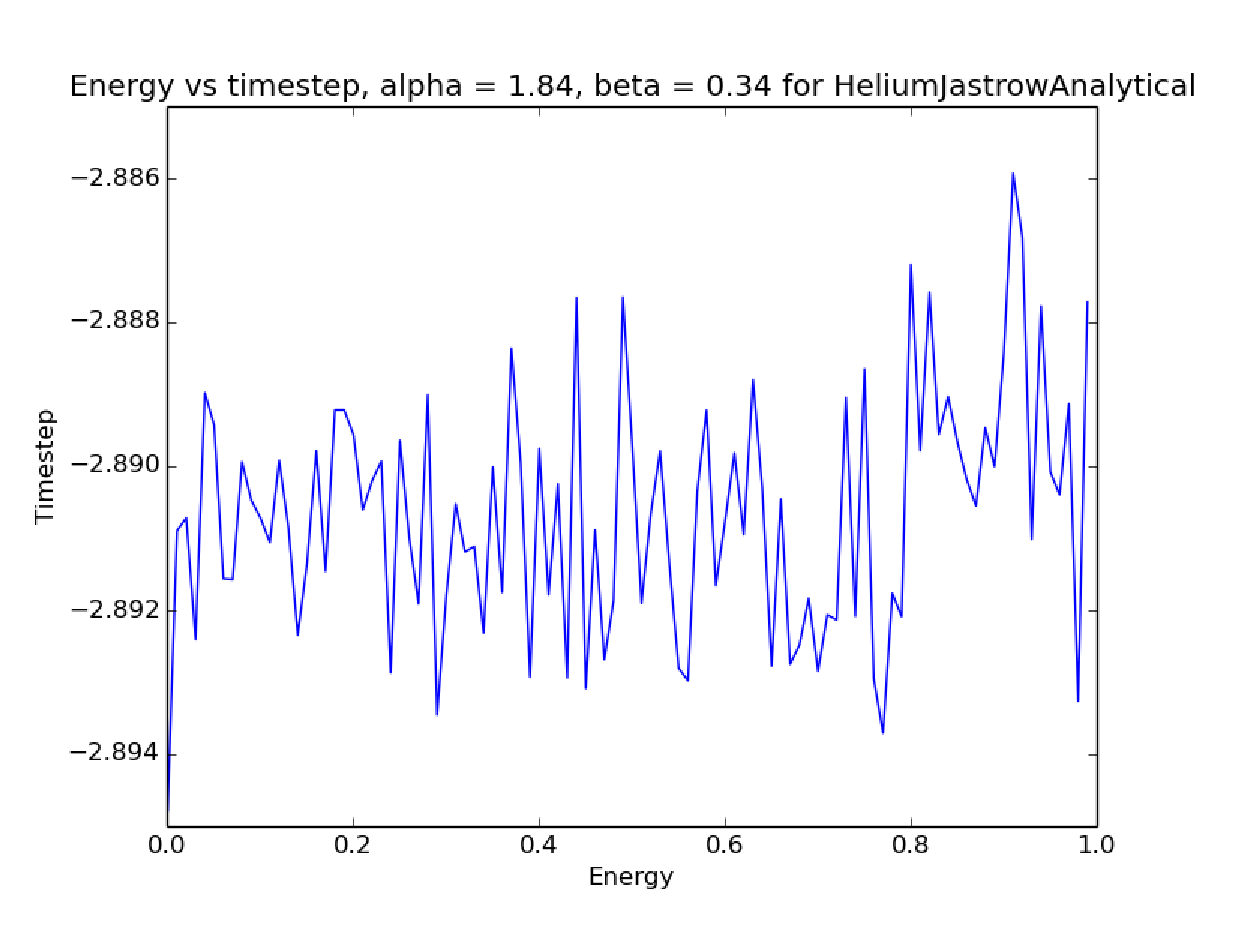
\includegraphics[width=0.45\linewidth]{../figures/HeliumJastrowAnalyticalTimeEnergy}
				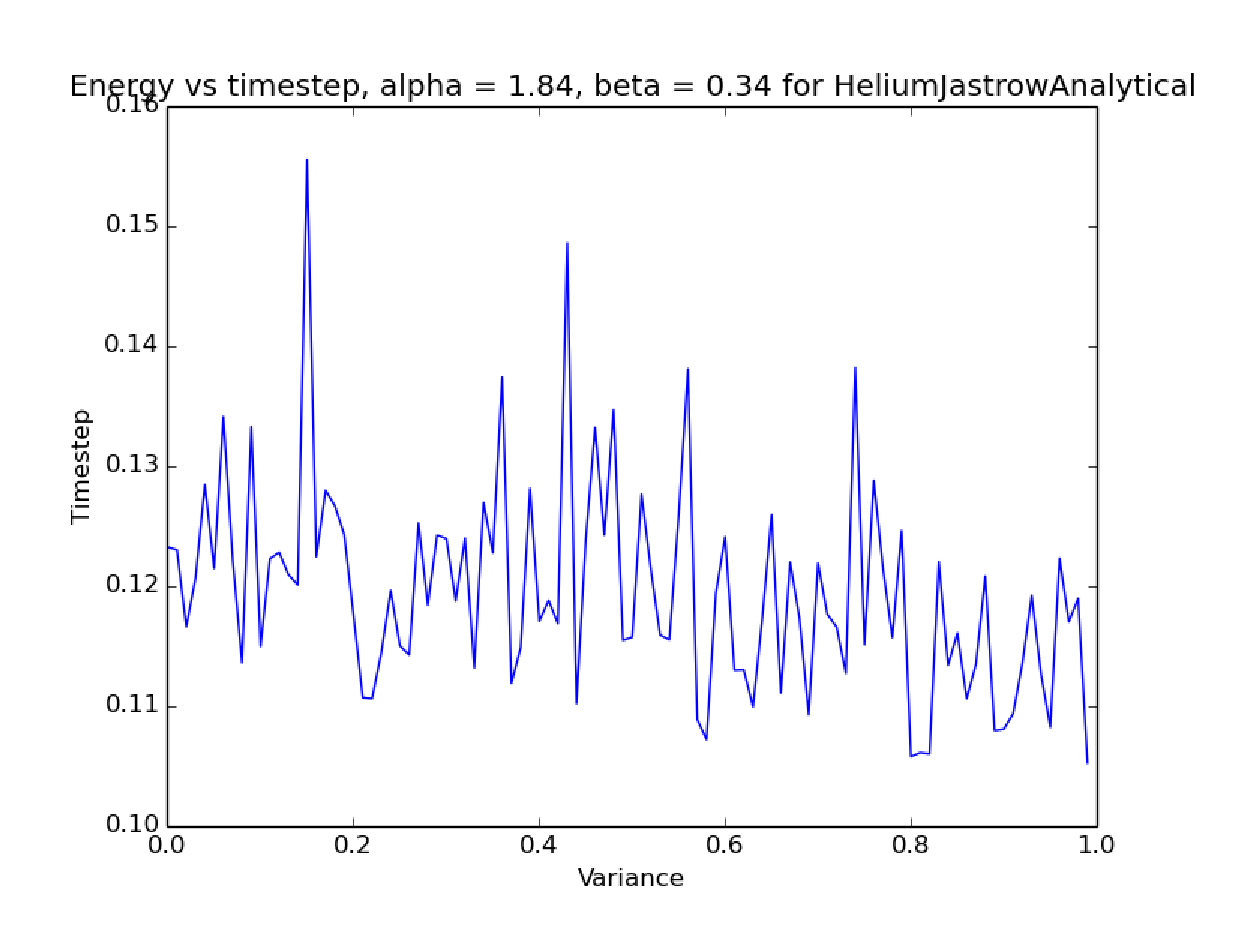
\includegraphics[width=0.45\linewidth]{../figures/HeliumJastrowAnalyticalTimeVariance}
				\protect\caption{Plots for Helium $\psi_{T}$ for the energy versus the timestep, and the variance versus the timestep.}
				\label{fig:HeliumTimestep}
			\end{figure}


		\subsubsection{Bisection method and GTOs}

		Using GTOs we can nearly reproduce the energies we get from using Slater Type Orbitals, although we are unable to reach quite the same energy. This is due to the GTOs being an imperfect representation of the STOs. Using GTOs in stead of STOs is also considerably slower, as we see in \ref{tab:AtomsGTO}. This can be due to inefficient code, and there is also room for improvements by calculating analytical derivatives of the GTOs. However using GTOs reduces the variables to only $\beta$, thus we don't have to look for energy minima by varying $\alpha$. This means that it is possible to easily use a gradient method to more efficiently find the variable that gives minimum energy.

		

	\subsection{Variational Monte Carlo calculations of the Beryllium and Neon atoms}

	We attempt to solve the ground state energy for the Beryllium atom and Neon atom using a Variational Monte Carlo calculation with importance sampling. We have used the trial functions \eqref{eq:BerylliumTrialFunction} for Beryllium and \eqref{eq:NeonTrialFunction} for Neon which uses $\alpha$ and $\beta$ as variational parameters.

	For Beryllium we have the Alpha and Beta values $\alpha=4.0$ and $\beta=0.31$. We use $10^{7}$ cycles and find the energy to be $-14.3902$ au, with a variance of $9.08566 \times 10^{-4}$.
	For Neon, with $10^{6}$ cycles, we get an energy of $-127.875$ au with a variance of $0.0131537$.

	From reseach papers we find the value for energy in the ground state
	of Beryllium to be $-14.667$ au \parencite{Koput_2011_PCCP}  and the value
	for energy in the ground state of Neon to be \(-128.928\) au \parencite{Binkley_1975}.
	In \cref{tab:EnergyAlphaBetaReference} we compare results
	obtained with our Variational Monte Carlo method with results from
	various research papers.

	\subsubsection{Alpha and Beta Values}

		\begin{figure}
			\centering \includegraphics[width=0.45\linewidth]{../figures/Beryllium_alpha_beta_energy}
			\centering \includegraphics[width=0.45\linewidth]{../figures/Beryllium_alpha_beta_variance}
			\protect\caption{Energy (left) and variance (right) for different Alpha and Beta values for Beryllium, using $10^{6}$ cycles.}
			\label{fig:alpha_beta_comparison_beryllium}
		\end{figure}

		\begin{figure}
			\centering \includegraphics[width=0.45\linewidth]{../figures/Neon_alpha_beta_energy}
			\centering \includegraphics[width=0.45\linewidth]{../figures/Neon_alpha_beta_variance}
			\protect\caption{Energy (left) and variance (right) for different Alpha and Beta values for Neon, using $10^{5}$ cycles.}
			\label{fig:alpha_beta_comparison_neon}
		\end{figure}

		To find optimal Alpha and Beta values for the atoms we run VMC with ranges of different values for \(\alpha\) and \(\beta\). The resulting plots of variance and energy for different combinations are given in figure \ref{fig:alpha_beta_comparison_beryllium} for Beryllium and figure \ref{fig:alpha_beta_comparison_neon} for Neon. The optimal values are shown in table \ref{tab:EnergyAlphaBetaReference}. As VMC runs slowly for Neon, because it has 10 electrons, we were only able to run over the range of Alpha and Beta values with $10^{5}$ cycles. This is reflected in the higher variance, and the spikes in the variance plot.

		\begin{table}
			\center %
			\begin{tabular}{|c|c|c|c|c|c|c|}
				\hline 
				Atom  & $\alpha$ & $\beta$ & Cycles & VMC {[}au{]} & Variance & Reference energy {[}au{]} \tabularnewline
				\hline 
				Helium & $1.843$ & $0.34$ & $10^{8}$ & $-2.89012$ & $7.76888\times10^{-5}$ & $-2.9037$\tabularnewline
				\hline 
				Beryllium  & $4.0$ & $0.31$ & $10^{7}$ & $-14.3902$  & $0.000908566$ & $-14.667$ \tabularnewline
				\hline 
				Neon  & $10.22$ & $0.091$ & $10^{6}$ & $-127.875$ & $0.0131537$ & $-128.928$ \tabularnewline
				\hline 
			\end{tabular}\protect\caption{Comparison of energies resulting from our Variational Monte Carlo method with
			energies found in research papers \parencite{Koput_2011_PCCP} \parencite{Binkley_1975}. The values for \(\alpha\) and \( \beta \) where found by doing running Monte Carlo calculation over a mesh of different \(\alpha\) and \( \beta \) values. The run with the lowest energy gave the \(\alpha\) and \(\beta\) values.}
			\label{tab:EnergyAlphaBetaReference} 
		\end{table}


	\subsubsection{Speedup with MPI}
		\begin{table}
			\center
			\begin{tabular}{| c | c| c| c| c|}
				\hline
					\textbf{Num. of processes} &	1	&	2	&	3	&	4
				\\ \hline
				\textbf{Speedup}	&	1.0	&	1.97	&	2.90	&	3.35
				\\	\hline
			\end{tabular}
			\caption{MPI speedup}
			\label{tab:MPI_speedup}
		\end{table}

		\begin{figure}
			\centering \includegraphics[width=0.45\linewidth]{../figures/processor_number_time_comparison}
			\protect\caption{MPI speedup}
			\label{fig:MPI_speedup}
		\end{figure}

		It is desirable to have a speedup as close as possible to the number of processors used. The speedup measured by our VMC program running 1, 2, 3 and 4 is shown in table \ref{tab:MPI_speedup} and figure \ref{fig:MPI_speedup}. We see that the speedup is good for 2 and 3 processes, but for 4 processes suffers somewhat because it also have to run the OS and other programs.


		\begin{table}
			\center %
			\begin{tabular}{|c|c|c|c|c|c|c|c|}
				\hline 
				Atom  & $\beta$ & Cycles & VMC {[}au{]} & Variance & Ref. energy {[}au{]} & GTO [s] & STO [s] \tabularnewline
				\hline 
				Helium &  $0.34$ & - & - & - & $-2.9037$ & - & - \tabularnewline
				\hline 
				Beryllium  &  $0.109375$ & $7\times 10^{7}$ & $-14.0182$ & $0.00203359$ & $-14.667$ & $48321$ & $4141$ \tabularnewline
				\hline 
				Neon  & $0.091$ & - & - & - & $-128.928$ & - & - \tabularnewline
				\hline 
			\end{tabular}\protect\caption{ Comparison of energies found using bisection method with the refenrence energy \parencite{Koput_2011_PCCP} \parencite{Binkley_1975} and comparison of the time used running the computation with the given number of cycles using GTOs and STOs.}
			\label{tab:AtomsGTO} 
		\end{table}	
	

\section{Conclusions and discussion}
	\subsection{Critique on the exercise}


\appendix

\section{Program overview}

	\begin{figure}
		\begin{tikzpicture}[%
		    >=triangle 60,              % Nice arrows; your taste may be different
		    start chain=going below,    % General flow is top-to-bottom
		    node distance=6mm and 45mm, % Global setup of box spacing
		    every join/.style={norm},   % Default linetype for connecting boxes
		    ]
		% ------------------------------------------------- 
		% A few box styles 
		% <on chain> *and* <on grid> reduce the need for manual relative
		% positioning of nodes
		\tikzset{
		  base/.style={draw, on chain, on grid, align=center, minimum height=4ex},
		  proc/.style={base, rectangle, text width=10em},
		  test/.style={base, diamond, aspect=2, text width=5em},
		  term/.style={proc, rounded corners},
		  % coord node style is used for placing corners of connecting lines
		  coord/.style={coordinate, on chain, on grid, node distance=6mm and 45mm},
		  % nmark node style is used for coordinate debugging marks
		  nmark/.style={draw, cyan, circle, font={\sffamily\bfseries}},
		  % -------------------------------------------------
		  % Connector line styles for different parts of the diagram
		  norm/.style={->, draw, lcnorm},
		  free/.style={->, draw, lcfree},
		  cong/.style={->, draw, lccong},
		  it/.style={font={\small\itshape}}
		}
		% -------------------------------------------------
		% Start by placing the nodes
		\node[proc, densely dotted, it] (init) {Initialize solver};
		\node[term, join] (split)      {Split into several threads for multi core};
		\node[term, join] (position)      {Suggest move};
		\node[term, join] (SD) { Compute/update \( |D| \) };
		\node[term, join ] (metro) {Compute Metropolis Ratio};
		\node[test, densely dotted , join ]	(test)	{\(R \ge r\)};
		\node[term]	(new_pos)	{\(\vb{r}^{old} = \vb{r}^{new}\)};
		\node[term, join ]	(energy)	{ Store \(E_L\) };
		\node[test, densely dotted ,join ]	(last)	{Last cycle?};
		\node[term]	(end)	{Collect samples};


		%Setting up the nodes on the side
		\node [term, right=of SD] (trialfunction) {Compute \( \psi_T(\vb{r}) \)};
		\node [term, left=of SD] (quantum) { Compute  Quantumforce};
		\node[term, left=of test] (old_pos) {Keep \(  \vb{r}^{old} \)};
		\node [coord, left=of new_pos] (c1)  {};    
		\node[coord, right=of last]	(around1){};
		\node[coord, right=of around1] (around2) {};
		\node[coord, right=of position]	(around3){};
		\node[coord, right=of around3]	(around4){};


		%Draw new links between boxes
		% \path (SD.south) to node [near start, xshift=1em] {$y$} (quantum);
		\draw [->,lcnorm] (SD.west) -- (quantum);
		\draw [->,lcnorm] (SD.east) -- (trialfunction);
		\draw [->, lcnorm] (quantum.south) -- (metro);
		\draw [->, lcnorm] (trialfunction.south) -- (metro);
		\draw [*->, lccong, , dotted] (test.west) -- (old_pos);
			\path (test.west) to node [ yshift = -1em] {no} (old_pos);
		\draw [*->, lcfree, dotted] (test.south) -- (new_pos);
			\path (test.south) to node [xshift = -1em]{yes} (new_pos);

		\draw [-, lcnorm] (old_pos.south) -- (c1);
		\draw [->, lcnorm] (c1.south) -- (energy);

		\draw[*-, lccong, dotted] (last.east) -- (around2);
			\path (last.east) to node [yshift = -1em] {no} (last);
			\draw[-, lccong, dotted] (around2.east) -- (around4);
			\draw[->, lccong, dotted] (around4) -- (position);

		\draw [*->, lcfree, dotted] (last.south) -- (end);
			\path (last.south) to node [xshift = -1em]{yes} (new_pos);


		\end{tikzpicture}
		\caption{Schematic overview over the workflow of the VMC solver}
		\label{fig:schematic}
	\end{figure}
\section{Class structure}
	\begin{figure}
		\begin{tikzpicture}[%
			    >=triangle 60,              % Nice arrows; your taste may be different
			    start chain=going below,    % General flow is top-to-bottom
			    node distance=6mm and 45mm, % Global setup of box spacing
			    every join/.style={norm},   % Default linetype for connecting boxes
			    ]
			% ------------------------------------------------- 
			% A few box styles 
			% <on chain> *and* <on grid> reduce the need for manual relative
			% positioning of nodes
			\tikzset{
			  base/.style={draw, on chain, on grid, align=center, minimum height=4ex},
			  proc/.style={base, rectangle, text width=10em},
			  test/.style={base, diamond, aspect=2, text width=5em},
			  term/.style={proc, rounded corners},
			  % coord node style is used for placing corners of connecting lines
			  coord/.style={coordinate, on chain, on grid, node distance=6mm and 45mm},
			  % nmark node style is used for coordinate debugging marks
			  nmark/.style={draw, cyan, circle, font={\sffamily\bfseries}},
			  % -------------------------------------------------
			  % Connector line styles for different parts of the diagram
			  norm/.style={->, draw, lcnorm},
			  free/.style={->, draw, lcfree},
			  cong/.style={->, draw, lccong},
			  it/.style={font={\small\itshape}}
			}

			%Center column
			\node[term, fill=lcfree!25,  align=center] (solver) {VMCSolver};
			\node[coord]	(blank)	{};
			\node[term] (trialfunction)	{Trialfunction};
				\draw[->, lcnorm]	(solver.south) -- (trialfunction);
			\node[term, join]	(diff)	{He, Be, Ne, H\(_2\) or Be\(_2\)};


			%Sides with lines drawn
			\node[term, right=of blank] (derivatives) {Derivatives};
				\draw[->, lcnorm] (solver.east) -- (derivatives.west);

			\node[term, left=of blank] 	(slater)	{SlaterDeterminant};
				\draw[->, lcnorm] (solver.west) -- (slater.east);

			%Dotted lines between the connected classes
			\draw[-, lcfree, densely dotted] (slater.east) -- (derivatives.west);
			\draw[-, lcfree, densely dotted] (slater.east) -- (trialfunction.west);
			\draw[-, lcfree, densely dotted] (trialfunction.east) -- (derivatives.west);

		\end{tikzpicture}

		\caption{Class and subclass structure used by the program}
		\label{fig:classes}
	\end{figure}

	\section{Verification of the model}
	To ensure that the program produces valid results as it gets more complicated we have implemented several different tests of smaller parts of the program that all should be met if the VMC solver is functioning properly. This section consists of a list of the different tests.
		\subsection{Verification of the general Monte Carlo method}
			Since the wavefunction for a Hydrogen atom can be calculated analytically, see equation \eqref{eq:hydrogen}, a Monte Carlo calculation with that wavefunction should return an exact value for the energy.

			\begin{align}
				 \Psi(\rho ) = \alpha \rho e^{-\alpha\rho} \qquad \text{ With  local energy: } \qquad E_{L} (\rho) = - \frac{1}{\rho} - \frac{\alpha}{2} \left( \alpha - \frac{2}{\rho} \right) \label{eq:hydrogen}
			\end{align}

			So a VMC calculation runrun with a Hydrogen atom with \(\alpha = 1\) it should produce an energy of exactly \( -0.5\) with \(0\) variance. 

		%Need to check up some stuff when including this.
		\subsection{Verification of the Slater determinant and the laplacian Slaterdeterminant ratio}
			\label{sec:slaterVerification}
			To verify the Slater determinant part of the trialfunctions we consider the atoms without any electron-electron interactions. Then it is a one-body system like hydrogen and can be calculated analytically, see \cite{griffiths2005introduction},  and we get exact wavefunctions and energy with \(0\) variance. 

			\begin{table}
			\begin{center}
				\begin{tabular}{| c | c |}
				\bottomrule
				Atom & Energy
				\\ \hline
				Hydrogen 	& \( E_{min} = -\frac{1}{2} \)
				\\ \hline
				Helium 		& \( E_{min} = -4\)
				\\ \hline Beryllium		& \( E_{min} = -20 \)
				\\ \hline Neon		& \( E_{min} = -200 \)
				\\ \toprule
				\end{tabular}
			\end{center}
			\caption{Ground states for the different atoms without electron-electron interaction}
			\end{table}

			In this case, where the correlation derivatives disappear, the kinetic part of the local energy gets simplified, from \eqref{eq:kineticRatio}, to the following

			\[\frac{\nabla^2 \Psi_T}{\Psi_T} = \frac{\nabla^2 |D_\uparrow|}{|D_\uparrow|} + \frac{\nabla^2 |D_\downarrow|}{|D_\downarrow|}  \]

			To reproduce the correct results both the Slater determinant and it's laplacian needs to be correct.

		\subsection{The gradient}
			\label{sec:gradientVerification}
			The gradient is used in the calculation of the quantum force, and all it's components is used in the calculation of the so by testing that this is correctly reproduced we get an inclination several terms are correct, \(\frac{\nabla |D_\uparrow|}{|D_\uparrow|} \), \( \frac{\nabla |D_\downarrow|}{|D_\downarrow|} \) and \( \frac{\nabla \Psi_C}{\Psi_C} \).

			The wavefunctions should be correct due to the earlier test, \ref{sec:slaterVerification}, so a numerical derivation of the trialfunction should produce a correct gradient, which is then used to test the analytical version against.


			\textbf{NB!!!!!!!!!!!!!! Does not pass at the moment...... Not sure why}

		\subsection{The correlation laplacian}
			\label{sec:laplacianCorrelationVerification}

			Due to the earlier two tests, \ref{sec:slaterVerification} and \ref{sec:gradientVerification}, we can be fairly certain that all the terms except the laplacian-correlation-ratio, \(\frac{\nabla^2\Psi_C}{\Psi_C}\) in the local energy equation \eqref{eq:kineticRatio} is correct. So by then comparing the analytical version of the local energy to the numerical version we can verify that the last term is also correct.

		\subsection{Local Energy in Helium}
			For Helium we have a complete closed expression for the local energy, \(E_l\) \eqref{eq:heliumLocalEnergy}, we use this to check that the local energy calculation, see "Efficient calculation of stuff chapters"!!!!!!!!!, used on the more complicated atoms  also replicates the local energy for the simpler atom which it does. 


		\subsection{Verification of correlation gradient}
			The correlation gradient ratio is checked by calculating what calculating it directly for Helium, and then comparing this value against value produced by the program.

			Let us consider the gradient ratio of the Padè-Jastrow factor in Helium, \(\frac{\nabla\psi_C(\vb{r}_{12})}{\psi_C(\vb{r}_{12})}\) with \(\psi_C(\vb{r_{12}}) = e^{\frac{r_{12}}{2(1+\beta r_{12})}}\). Using the results from equation \eqref{eq:gradient_ratio_Jastrow} on Helium for the first electron we get

			\begin{align}
				\left[\frac{\nabla\Psi_C}{\Psi_C} \right]_1 &= \frac{1}{\Psi_c} \pdv{\Psi_C}{x_k} = \frac{\vb{r_{12}}}{r_{12}}\pdv{}{r_{12}}\left( \frac{r_{12}}{2(1+\beta r_{12})} \right) - \frac{\vb{r_{21}}}{r_{21}}\pdv{}{r_{21}}\left( \frac{r_{21}}{2(1+\beta r_{21})} \right)
				\\
				&= 2\frac{\vb{r_{12}}}{r_{12}}\pdv{}{r_{12}}\left( \frac{r_{12}}{2(1+\beta r_{12})} \right)
				\\
				&= \frac{\vb{r_{12}}}{r_{12}} \frac{1}{(1+\beta r_{12})^2}
			\end{align}

			Testing that the program reproduces this for the helium atom indicates the \(\frac{\nabla \Psi_C}{\Psi_C}\) is being calculated correctly.

		\subsection{Hydrogen Molecule}
			\textbf{NB!!!!!!!!!!!!!! Write this}\\




\bibliography{bibliography}
\bibliographystyle{plain}


\end{document}